\documentclass[a4paper,11pt,DIV=11]{scrartcl}
\usepackage[utf8]{inputenc}
\usepackage[version=4]{mhchem}
\usepackage[ngerman]{babel}
\usepackage{amsfonts, amsmath, amssymb}
\usepackage{graphicx}
\usepackage{float}
\parindent0pt

\title{Transmissions-Elektronen-Mikroskopie}
\author{Adrian Messow, Sven Mehrkens \\
Tutor: ???}
\date{Durchführung: 14.12.2017 \\ Abgabe: ??? }

\begin{document}
\maketitle
\section{Einführung}
In diesem Versuch werden die Grundlagen des Transmissionselektronenmikroskops (TEM) vermittelt. Dabei werden nach einer grundlegenden Justierung die Beugungsbilder im Hellfeld und Dunkelfeld an einer GaAs-Probe aufgenommen und indiziert. Durch Aufnahmen von InGaAs-Quantentrögen wird anschließend einerseits über die Intensitätsverteilung und andererseits über die Gitterkonstanten die Indiumkonzentration bestimmt.

\section{Theoretische Grundlagen}
Transmissionselektronenmikroskope erreichen eine Auflösung die im Sub-\(\mathrm{\mathring{A}}\)-Bereich liegt. Dies liegt an der Verwendung von Elektronen zur Bildgebung, anstatt von Photonen in herkömlichen Lichtmikroskopen. Dabei werden Elektronen aus einem Filament heraus beschleunigt und werden über Linsensysteme auf die Probenoberfläche fokussiert. Die transmittierten Elektronen werden über geeignete Beobachtungssysteme sichtbar gemacht. Das Auflösungsvermögen wird durch das Raleigh-Kriterium beschrieben und kann bei kleinen Winkelabweichungen von \(\alpha<1^\circ\) beschrieben werden durch \(\delta > 60\lambda\). Für eine typische Bechleunigungsspannung von \(100\,\mathrm{kV}\) ergibt sich eine Auflösung von \(0,2\,\mathrm{nm}\). Dabei wird die Wellenlänge des Elektrons durch die \textit{de Broglie Wellenlänge} für relativistische Teilchen beschrieben: 
\begin{align}
\lambda = \frac{h}{\sqrt{2m_\mathrm{0}eV(\frac{1+eV}{2m_\mathrm{0}c^2})}}
\end{align}
Mit \(h\) dem planck'schen Wirkungsquantum, \(m_\mathrm{0}\) der Ruhemasse des Elektrons, \(c\) der Lichgeschwindigkeit und \(eV\) der Energie des Elektrons in Elektronenvolt.
Zwei Bildgebungsarten sich möglich. Das erste ist das Beugungsbild, hier wird das reziproke Gitter des Kristalls abgebildet. Das zweite ist das Realbild (Abb. \ref{Strahlengang}).
\begin{figure}[H]
\center
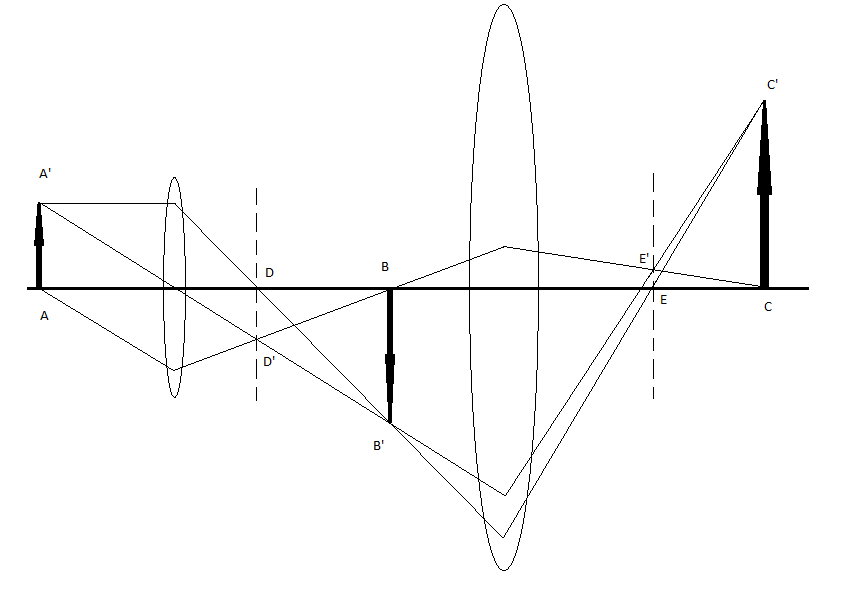
\includegraphics[width=\textwidth]{Strahlengang.png}
\caption{Schematische und vereinfachte Darstellung des Strahlenganges zur Entstehung der zwei Bildarten. Realbilder bei BB' und CC'. Beugungsbilder bei DD' und EE'.}
\label{Strahlengang}
\end{figure}

	
\section{Versuchsaufbau und Versuchsdurchführung}

\section{Auswertung}

\section{Zusammenfassung}

\section*{Anhang}

\end{document}